
\documentclass[8pt]{beamer}

\usepackage[utf8]{inputenc} 
\usepackage[T1]{fontenc}
\usepackage{lmodern}
\usepackage{graphicx}
\usepackage[french]{babel}
\usepackage[absolute,overlay]{textpos}
\usepackage{textpos} % package for the positioning

\usepackage{animate}

\usetheme{Darmstadt}

\setcounter{tocdepth}{1}
\AtBeginSection[]
{
	\begin{frame}
		\tableofcontents[currentsection]
	\end{frame}
}


% position the logo
\addtobeamertemplate{frametitle}{}{%
\begin{textblock*}{100mm}(11.5cm,8cm)

\includegraphics[height=1.3cm,width=1.3cm,keepaspectratio]{./images/logo.png}
\end{textblock*}}


\setbeamertemplate{footline}[frame number]
\beamertemplatenavigationsymbolsempty

\begin{document}

\title{GDB ou comment débugger un programme intelligemment}
\author{Corentin DESCAMPS - Marian GAPPA}

\maketitle

\begin{frame}
\tableofcontents
\end{frame}


\section{GDB, the GNU project DeBugger} % (fold)
\label{sec:gdb_the_gnu_project_debugger}

\subsection{GDB - Introduction} % (fold)
\label{sub:gdb_introduction}

\begin{frame}
\frametitle{GDB - Qu'est ce que c'est ?}

\onslide<1->\begin{block}{Définition}
GDB, GNU project DeBugger, vous autorise à voir ce qui se passe à l'intérieur d'un autre programme pendant son execution, ou lors de son arrêt innopiner de celui-ci.
\end{block}

\onslide<1->GDB a 4 principaux objectifs:
\begin{enumerate}
	\onslide<2->\item Commencer votre programme, en spécifiant tout ce qui peut affecter son déroulement.
	\onslide<3->\item Arrêter votre programme à des endroits, ou à des conditions, spécifiés.
	\onslide<4->\item Voir l'état global de votre programme quand celui-ci s'arrête.
	\onslide<5->\item Changer des variables dans votre programme, afin d'expérimenter la correction d'un bug.
\end{enumerate}

\end{frame}


\begin{frame}
\frametitle{GDB - Pourquoi l'utiliser ?}

\onslide<1->Un ensemble de raison non exaustif :
\begin{itemize}
	\onslide<2->\item Voir les problèmes de raisonnement facilement.
	\onslide<3->\item Observer l'origine possible d'une erreur de segmentation.
	\onslide<4->\item Tester son programme.
	\onslide<5->\item Support les langages Ada, C, C++, Objectif-C, Pascal...
	\onslide<6->\item Créer par Richard Stallman.
	\onslide<7->\item Ne pas être obliger de mettre des printf partout dans le code pour regarder l'état des variables.
\end{itemize}
\end{frame}


\begin{frame}
\frametitle{GDB - Pourquoi l'utiliser ?} 

\begin{figure}[]
	\centering
	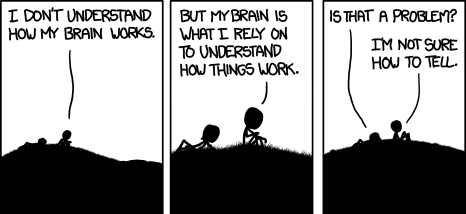
\includegraphics[width=11cm]{./images/debugger.png}
	\caption{XKCD 1163}
	\label{fig:figure1}
\end{figure}

\end{frame}

\begin{frame}
\frametitle{GDB - Des autres debbuger ?}

\onslide<1->Liste de débugger :
\begin{itemize}
	\onslide<2->\item Mtrace
	\onslide<3->\item Memwatch
	\onslide<4->\item Bashdb
	\onslide<5->\item CodeView
	\onslide<6->\item Dmalloc
	\onslide<7->\item Electric Fence
	\onslide<8->\item Valgrind
	\onslide<9->\item DDD
	\onslide<10->\item gdb-mode
\end{itemize}

\end{frame}

% subsection gdb_introduction (end)


\subsection{GDB - Utilisation} % (fold)
\label{sub:gdb_utilisation}

\begin{frame}
\frametitle{GDB - Préparer son éxécutable}

\onslide<1->\begin{block}{Options de compilation de GCC}
	gcc -O0 -g file.c -o executable\\
	gcc -O0 -ggdb3 file.c -o executable
\end{block}

\onslide<2->\begin{alertblock}{À ne pas faire lors d'un rendu}
Laisser l'option de debug actif dans le Makfile lors du rendu.
\end{alertblock}

\end{frame}


\begin{frame}
\frametitle{GDB - Lancer son programme dans GDB}
\onslide<1->\begin{block}{Éxecuter son programme sans arguments}
	gdb executable
\end{block}

\onslide<2->\begin{block}{Éxecuter son programme avec des arguments}
	gdb --args executable arg1 arg2
\end{block}

\onslide<3->\begin{block}{Lancer GDB avec une semi-interface}
	gdb -tui executable
\end{block}

\end{frame}


\begin{frame}
\frametitle{GDB - Éxecuter son programme dans GDB}

Commande d'éxécution jusqu'à l'arrêt du programme ou à un point d'arrêt :
\begin{itemize}
	\onslide<2->\item run
	\onslide<3->\item run arg1 arg2
	\onslide<4->\item r
\end{itemize}

\end{frame}


\begin{frame}
\frametitle{GDB - Qu'est ce que des points d'arrêt ?}

\begin{block}{Définition}
	Pour contrôler l'exécution d'un programme ou éxaminer l'état de variables, on place des points d'arrêt.
\end{block}

\end{frame}


\begin{frame}
\frametitle{GDB - Mettre des points d'arrêt}

Commande permettant d'arrêter l'exécution d'un programme :
\begin{itemize}
	\onslide<2->\item break [file.c]:line
	\onslide<3->\item break [file.c]:function
	\onslide<4->\item b [file.c]:line
	\onslide<5->\item b [file.c]:line if condition
	\onslide<6->\item watch variable
\end{itemize}

\end{frame}


\begin{frame}
\frametitle{GDB - Continuer son exécution I}

\begin{block}{Continuer jusqu'au prochain point d'arrêt}
	continue\\
	c
\end{block}

\onslide<2->\begin{block}{Continuer ligne par ligne}
	next\\
	next [next\_line]\\
	n [next\_line]
\end{block}

\onslide<3->\begin{block}{Continuer précisement ligne par ligne}
	step\\
	step [next\_line]\\
	s [next\_line]\\
\end{block}

\end{frame}


\begin{frame}
\frametitle{GDB - Continuer son éxécution II}
    
\onslide<4->\begin{block}{Continuer jusqu'à la sortie de fonction}
	finish\\
	f
\end{block}

\onslide<5->\begin{block}{Continuer jusqu'à une ligne}
	until line\\
	u line
\end{block}

\end{frame}


\begin{frame}
\frametitle{GDB - Autres actions les points d'arrêt}

\begin{block}{Lister les points d'arrêt}
	info break\\
	info break [breaknumber]
\end{block}

\begin{block}{Supprimer un (ou des) point(s) d'arrêt}
	clear line\\
	clear function\\
	delete [breaknumber]\\
	delete\\
\end{block}

\end{frame}


\begin{frame}{GDB - Affichage}

\begin{block}{Affichage d'une varible}
	print variable
\end{block}


\onslide<2->\begin{block}{Affichage selon un format}
	p/format variable\\
	p/format expression\\
	format = [x | d | u | o | t | a | c | f]
\end{block}

\onslide<3->\begin{block}{Affichage de la pile d'exécution}
	backtrace
\end{block}

\end{frame}


\begin{frame}{GDB - Quitter GDB}
	\begin{block}{Quitter GDB}
		quit
	\end{block}
\end{frame}

% subsection gdb_utilisation (end)

\subsection{GDB - Vérification de la mémoire} % (fold)
\label{sub:gdb_v_rification_de_la_m_moire}

\begin{frame}{GDB - Vérifier les fuites de mémoires}
\begin{block}{Utilisation de GCC}
	gcc file.c -o executable -fsanitize=address
\end{block}
\end{frame}

% subsection gdb_v_rification_de_la_m_moire (end)


% section gdb_the_gnu_project_debugger (end)


\section{GCC - Vérification de la mémoire} % (fold)
\label{sec:gcc_v_rification_de_la_m_moire}

\subsection{GCC - Vérifier les fuites de mémoire} % (fold)
\label{sub:gcc_v_rifier_les_fuites_de_m_moire}

\begin{frame}
\frametitle{GCC - Vérifier les fuites mémoires}
\begin{block}{Utilisation de GCC}
	gcc file.c -o executable -fsanitize=address
\end{block}
\end{frame}

% subsection gcc_v_rifier_les_fuites_de_m_moire (end)

% section gcc_v_rification_de_la_m_moire (end)

\section{Démonstration} % (fold)
\label{sec:d_monstration}

\subsection{Démonstration} % (fold)
\label{sub:d_monstration}

\begin{frame}
\frametitle{Démonstration}

Démonstration de GCC et de GDB

\end{frame}

% subsection d_monstration (end)

% section d_monstration (end)

\end{document}
